\documentclass[utf8]{beamer}
\usepackage{listings}
\usepackage[russian]{babel}
\usetheme{Malmoe}
\title{Анализ выходных данных для автономной системы}
\author {Кирилл Андреев}
\date{25 Октября 2011 г.}
\begin{document}
%--------------------------------------------------------------------------------
\begin{frame}
\titlepage
\end{frame}
%--------------------------------------------------------------------------------
\section {Введение}
%--------------------------------------------------------------------------------
\begin{frame}
\frametitle{Наиболее распространенные заблуждения}
\begin{itemize}
	\item Использование единственного прогона модели при анализе систем
	\item Предположение о независимости случайных величин, получаемых в ходе одного прогона модели
\end{itemize}
\end{frame}
\subsection{Процесс моделирования}
%--------------------------------------------------------------------------------
\begin{frame}
\frametitle{Наиболее распространенные заблуждения}
\begin{itemize}
	\item Использование единственного прогона модели при анализе систем
	\item Предположение о независимости случайных величин, получаемых в ходе одного прогона модели
\end{itemize}
\end{frame}
%--------------------------------------------------------------------------------
\begin{frame}
\frametitle{Процесс моделирования}
Пусть $Y_1, \ldots, Y_m$ -- стохастический процесс, реализуемый при прогонах модели.
$$
\textrm{Прогоны модели}
\underbrace{
\left\{
\begin{array}{ccccc}
y_{11}, & \ldots, & y_{1i} ,& \ldots, & y_{1m},\\
y_{21}, & \ldots, & y_{2i}, & \ldots, & y_{2m},\\
\vdots & &\vdots & &\vdots \\
y_{n1}, & \ldots, & y_{ni}, & \ldots, & y_{1m},\\
\end{array}
\right.
}_{\textrm{наблюдения в одном прогоне}}
$$
Строки матрицы соответствуют наблюдаемым величинам при \underline{различных прогонах модели} с использованием \underline{различных последовательностей входных случайных чисел}.
\begin{itemize}
	\item Внутри строки величины не независимы
	\item Внутри столбца величины независимы
\end{itemize}
\end{frame}
\subsection{Наличие начальных условий}
%--------------------------------------------------------------------------------
\begin{frame}
\frametitle{Наличие начальных условий}
\begin{itemize}
	\item $Y_1, Y_2, \ldots$ - выходной стохастический процесс
	\item Функция распределения наблюдаемой $F_i(y|I) = P(Y_i \leq y | I)$зависит от начальных условий $I$.
	\item $P(Y_I \leq y)$ -- вероятность того, что произойдет событие $\{Y_i \leq y\}$
	\item $F_i(y|I)$ -- переходное распределение выходного процесса в момент времени $i$ при начальных условиях $I$
		\begin{itemize}
			\item Функции различны при различных начальных условиях
			\item Функции различны в различные моменты времени
		\end{itemize}
	\item Предполагаем, что существует такое $i\rightarrow \infty$, при котором зависимость от начальных условий \emph{практически} исчезает
	\item  Установившееся состояние -- \underline{распределение} наблюдаемой величины перестает зависеть от времени.
	\item Скорость выхода на установившееся состояние зависит от начальных условий
\end{itemize}
\end{frame}
%--------------------------------------------------------------------------------
\begin{frame}
\frametitle {Выход на стационарное состояние}
\begin{center}
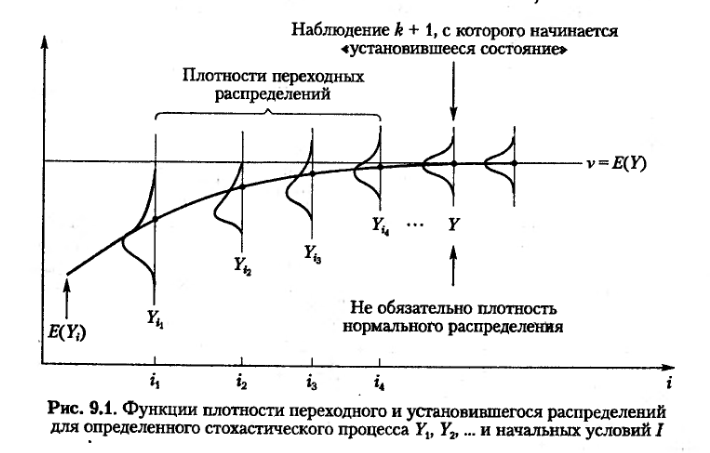
\includegraphics[width=\textwidth]{pic/9-2.png}
\end{center}
\end{frame}
%--------------------------------------------------------------------------------
\begin{frame}
\frametitle {Скорость схождения к стационарному состоянию}
\begin{center}
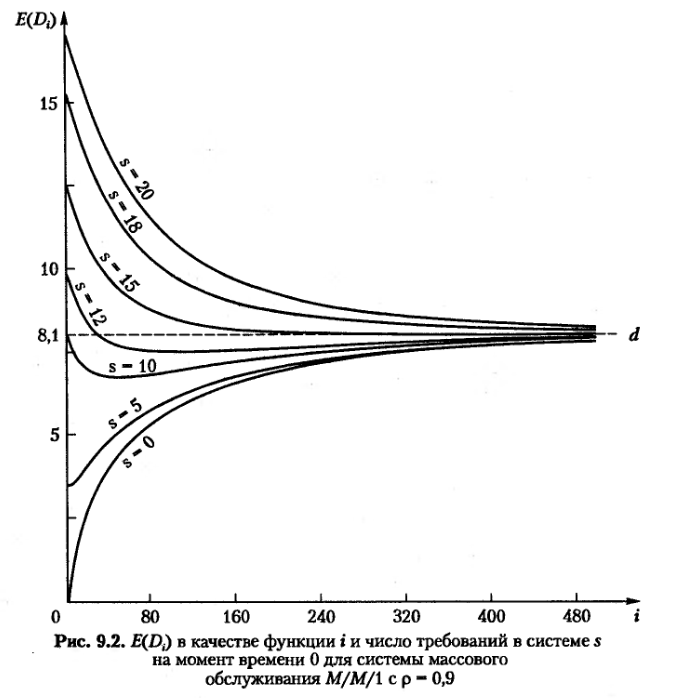
\includegraphics[width=0.6\textwidth]{pic/9-3.png}
\end{center}
\end{frame}
\subsection{Типы имитационного моделирования}
%--------------------------------------------------------------------------------
\begin{frame}
\frametitle{Типы имитационного моделирования}
\begin{itemize}
	\item Переходный режим имитационного моделирования -- наличие терминирующего события. Важен тщательный выбор начальных условий.
	\item Имитационное моделирование для непереходного режима -- невозможность определения терминирующего события, потенциально бесконечное время моделирования.
\end{itemize}

\end{frame}
%--------------------------------------------------------------------------------
\begin{frame}
\frametitle{Переходный режим имитационного моделирования}
\begin{itemize}
	\item Моделирование системы с конечным временем работы (рабочий день в банке)
	\item Моделирование боевых действий -- наличие терминирующего события (победа/поражение)
	\item Моделирование различных производственных циклов
\end{itemize}
\end{frame}
%--------------------------------------------------------------------------------
\begin{frame}
\frametitle{Непереходный режим имитационного моделирования}
\begin{itemize}
	\item Критерий оценки имитационной модели -- установившиеся параметры (если существуют) выходного распределения. Характеристики модели при этом считаются неизменными.
	\item Возможно наличие циклических установившихся параметров: пусть дан стохастический процесс $Y_1, Y_2, \ldots$ непрекращающегося процесса моделирования, в котором нет установившегося состояния. $Y_i^C$ - случайная величина, определенная в $i-$м цикле. Если случайные процессы в каждом цикле сопоставимы, и характеристики этих процессов сходятся, то их называют циклическими установившимися параметрами.
	\item Если параметры модели изменяются со временем, то возможно свести процесс к переходному.
\end{itemize}
\end{frame}

%--------------------------------------------------------------------------------
\begin{frame}
\frametitle{Типы имитационного моделирования}
\begin{center}
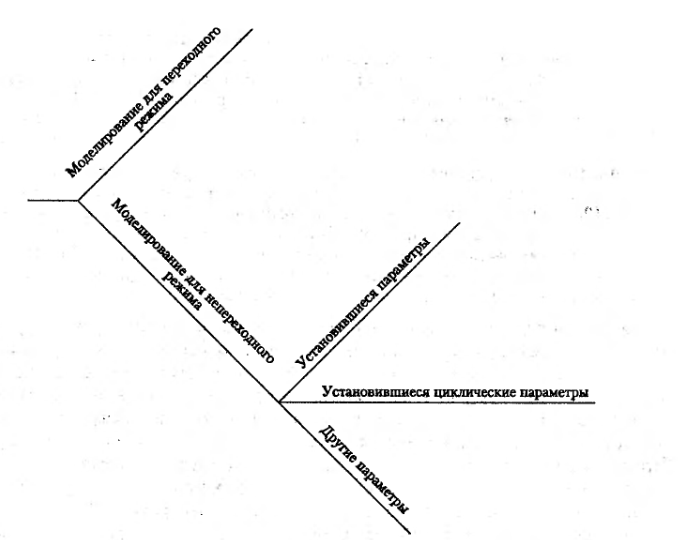
\includegraphics[width=.8\textwidth]{pic/9-4.png}
\end{center}
\end{frame}
%--------------------------------------------------------------------------------
\section{Статистический анализ при переходном режиме}
\subsection{Метод конечного объема выборки}
%--------------------------------------------------------------------------------
\begin{frame}
\frametitle{Оценка средних значений по результатам $n$ прогонов: предположения}
\begin{itemize}
	\item Выполняется $n$ независимых прогонов
	\item Существует одна оценка искомая оценка критерия (одна величина на один прогон), например среднее ожидание в очереди в банке за день.
	\item Существует $n$ независимых одинаково распределенных $X_j$, являющихся искомой оценкой 
\end{itemize}
\end{frame}
%--------------------------------------------------------------------------------
\begin{frame}
\frametitle{Оценка средних значений по результатам $n$ прогонов: точечная оценка и доверительные интервалы}
\begin{block}{Процедура с фиксированным объемом выборки: получение приближенного доверительного интервала}
Оценка среднего $\mu = E(X)$, где $X$ -- случайная величина, определенная при повторном прогоне. Тогда за $n$ прогонов имеем $X_1, \ldots, X_n$ -- независимые одинаково распределенные случайные величины. $\overline{X}(n)$ -- несмещенная оценка, а $100-\alpha$-процентный доверительный интервал тогда составит $\overline{X}(n)\pm t_{n-1, 1-\frac{\alpha}{2}} \sqrt{\frac{S^2(n)}{n}}$, где $S^2(n)$ -- выборочная дисперсия.
\end{block}
\begin{block}{Предположения в процедуре с фиксированным объемом выборки}
 \begin{enumerate}
 	\item Оцениваемые величины одинаково распределены
	\item Оцениваемые величины имеют гауссово распределение
\end{enumerate}
\end{block}
\end{frame}
%--------------------------------------------------------------------------------
\subsection{Метод получения заданной точности}
\begin{frame}
\frametitle{Механизмы получения заданной точности}
Сколько необходимо независимых прогонов модели для того, чтобы точно контролировать половину длины доверительного интервала?
\begin{itemize}
	\item Получение необходимого числа прогонов в предположении
  ``несущественного изменения'' выборочной дисперсии $S^2 (n)$
  \item Последовательная процедура получения заданной точности
\end{itemize}
В дальнейшем зависимость $\overline{X}$ от $n$ исчезает, так как $n$ -- случайная величина
\end{frame}
%--------------------------------------------------------------------------------
\begin{frame}
\frametitle{Получение числа прогонов при условии несущественного изменения дисперсии}
Пусть $\beta$ -- абсолютная погрешность $\overline{X}$, то есть $|\overline{X}-\mu| = \beta$.
Тогда доверительный интервал определен как:
$$
1-\alpha \approx P(\overline{X}-\textrm{половина длины} \leq \mu \leq \overline{X}+\textrm{половина длины})
$$
То есть с вероятностью $\alpha$\% \emph{среднее} значение наблюдаемой будет
лежать внутри доверительного интервала $\pm \beta$.

Приближенное необходимое число прогонов составит:
$$
n_{\alpha}^{\star}(\beta) = min \Big\{ i\geq n : t_{i-1, 1-\frac{\alpha}{2}}
\sqrt{\frac{S^2(n)}{i} \leq \beta} \Big\}
$$
По результатам $n$ первых прогонов оцениваем общее необходимое их
число и выполняем еще $n - n_{\alpha}^{\star}$ прогонов.
\end{frame}
%--------------------------------------------------------------------------------
\begin{frame}
\frametitle{Получение числа прогонов при условии несущественного
изменения дисперсии}
Пусть необходимо зафиксировать абсолютную погрешность $\gamma$, то
аналогичным образом можно получить:
$$
n_{r}^{\star}(\gamma) = min \Big\{ i\geq n :
\frac{t_{i-1, 1-\frac{\alpha}{2}}\sqrt{\frac{S^2(n)}{i}}}{|\overline{X}(n)|} \leq \frac{\gamma}{1+\gamma} \Big\}
$$
Недостатки метода: $\overline{X}(n)$ и $S^2(n)$ не могут быть точными
оценками соответствующих параметров генеральной совокупности.
\end{frame}
%--------------------------------------------------------------------------------
\begin{frame}
\frametitle{Последовательная процедура получения заданной точности}
Необходимо получить оценку $\mu$ с заданной относительной точностью
$\gamma \in (0, 1)$. Пусть изначально выполнено $n_0\geq2$ независимых
прогонов модели. Обозначим
$$
\delta (n, \alpha) = t_{n-1, 1-\frac{\alpha}{2}}\sqrt{\frac{S^2(n)}{n}}
$$
\begin{enumerate}
  \item Выполняем $n_0$ повторных прогонов модели и задаем $n = n_0$.
  \item Вычисляем $\overline{X}(n)$ и $\delta (n, \alpha)$ по $X_1, X_2, \ldots, X_n$
  \item Если $\delta (n, \alpha)\leq \overline{X}(n) \cdot \frac{\gamma}{1+\gamma}$, то используем $\overline{X}(n)$ как точечную оценку для $\mu$ и останавливаемся или повторяем процедуру иначе, выполняя $n+1$-й прогон модели.
\end{enumerate}
\end{frame}
%--------------------------------------------------------------------------------
\begin{frame}
\frametitle{Последовательная процедура получения заданной точности}
В результате $\alpha$\% доверительный интервал с относительной
точностью $\gamma$ составит:
$$
I(\alpha, \gamma) = [\overline{X}(n)-\delta (n, \alpha), \overline{X}(n)+\delta (n, \alpha)]
$$
\begin{block}{Выводы}
\begin{itemize}
  \item Второй способ, как правило, дает существенно большее необходимое число независимых прогонов модели, т.к. на основании малого количества начальных прогонов получаются неточные оценки.
  \item Обычно следует использовать $n_0 \geq 10, \gamma \leq 0.15$
\end{itemize}
\end{block}
\end{frame}
%--------------------------------------------------------------------------------
\subsection{Выводы}
\begin{frame}
\frametitle{Общие выводы}
\begin{itemize}
  \item Процедура с фиксированным объемом выборки хороша, когда
  точность не имеет принципиального значения. Если распределения
  существенно отличны от нормального, доверительный интервал может
  оказаться на самом шире, что нежелательно.
  \item Приблизительная оценка общего количества экспериментов хороша
  при ограниченных ресурсах на проведение эксперимента.
  \item Для получения точных оценок лучше пользоваться последовательной
  процедурой с $n_0 \geq 10, \gamma \leq 0.15$.
\end{itemize}
\end{frame}
%--------------------------------------------------------------------------------
\begin{frame}
\frametitle{Общие выводы}
\begin{itemize}
  \item Никогда не полагаться на результаты, полученные на основании
  менее пяти прогонов модели.
  \item Тщательно выбирать оцениваемые параметры. Наример - ожидаемая
  средняя задержка и ожидаемое количество клиентов по времени для
  одной или нескольких очередей.
  \item Тщательно подбирать начальные условия. Например -- работа
  банка после обеденного перерыва. Рекомендация: отдельно моделировать
  процесс выбора начальных данных.
\end{itemize}
\end{frame}
%--------------------------------------------------------------------------------

\section{Статистический анализ при непереходном режиме}
\subsection{Описание проблемы}
%--------------------------------------------------------------------------------
\begin{frame}
\frametitle{Статистический анализ установившихся параметров: проблема
запуска}
\begin{itemize}
  \item Пусть $Y_1, Y_2, \ldots$ -- стохастический процесс, полученный в
результате прогона модели в непереходном режиме.
  \item Предположим, что имеется установившееся состояние: $P(Y_i \leq
  y) = F_i() \rightarrow F(y) = P(Y\leq y)$, где Y -- установившаяся
  случайная величина с функцией распределения $F$.
  \item $\phi$ -- установившаяся характеристика $Y$ (например, среднее
  значение)
  \item Эта оценка отлична от действительной, т.к. мы не можем выбрать
  ``правильные'' начальные условия, то есть оценки смещены.
\end{itemize}

\end{frame}
%--------------------------------------------------------------------------------
\begin{frame}
\frametitle{Проблема начального переходного процесса}
Пусть необходимо оценить установившееся среднее $\nu = E(Y)$
$$
\nu = \lim_{i \rightarrow \infty} E(Y_i)
$$
Удаление начальных данных, снижающее смещение оценки:
$$
\overline{Y}(m, l) = \frac
                          {\sum_{i=l+1}^{m}Y_i}
                          {m-l}
$$
Данные, близкие к началу моделирования, могут оказаться
\emph{нехарактерными} для рассматриваемой системы.

Проблема начального переходного процесса в выборе $l$ и $m$ таких, чтобы получить необходимое качество получаемой оценки.
\end{frame}
%--------------------------------------------------------------------------------
\subsection {Графический метод Велча}
\begin{frame}
\frametitle{Описание метода Велча}
\begin{enumerate}
  \item Выполнение $n$ прогонов модели (более 5!), \emph{достаточно} длительных.
  \item Получение на основании нескольких прогонов средних показателей
  работы системы.
  \item Фильтрация высокочастотных колебаний методом оконной
  фильтрации:
$$
\overline{Y}_i(w) = \left\{
\begin{array}{ll}
\frac{\sum_{s=-w}^{w}\overline{Y}_{i+s}}{2w +1} & \textrm{если } i = w+1, \ldots, m-w\\
\frac{\sum_{s=-(i+1)}^{i-1}\overline{Y}_{i+s}}{2i -1} & \textrm{если } i = 1, \ldots, w\\
\end{array}
\right.
$$
  \item Строим график полученного скользящего среднего.
\end{enumerate}
\end{frame}
%--------------------------------------------------------------------------------
\begin{frame}
\frametitle{Описание метода Велча}
\begin{center}
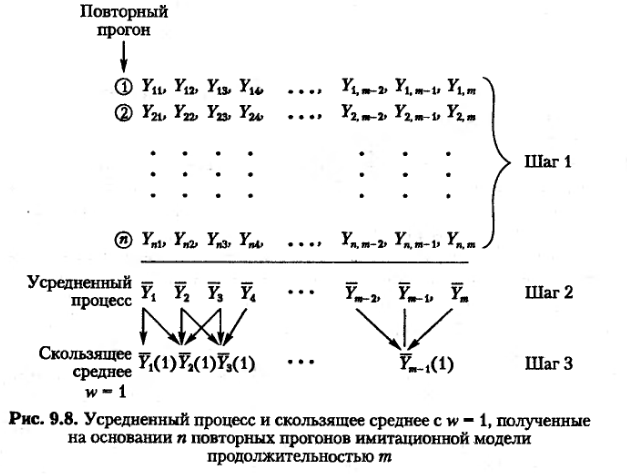
\includegraphics[width=0.8\textwidth]{pic/9-8.png}
\end{center}
\end{frame}
%--------------------------------------------------------------------------------
\begin{frame}
\frametitle{Общие рекомендации по применению метода}
\begin{itemize}
  \item Выбрать 5 или 10 прогонов, выбрать настолько большое $m$,
  насколько это целесообразно в практическом смысле. $m$  должно быть
  существенно больше ожидаемого значения $l$.
  \item Построить график $\overline{Y}_i(w)$ для нескольких значений
  окна $w$ и выбрать наименьшее значение, при котором соответствующий
  график будет ''достаточно ровным`` Больший размер окна больше
  сглаживает получаемый график $\Rightarrow$ слишком большое окно
  брать не стоит.
  \item Если не подходит ни одно выбранное значение окна, то стоит
  выполнить дополнительные прогоны и повторить процедуру.
\end{itemize}
\end{frame}
%--------------------------------------------------------------------------------
\begin{frame}
\frametitle{Общие рекомендации по применению метода}
\begin{itemize}
  \item Существуют более сложные оконные функции для получения результатов (Фильтры Калмана)
  \item Использование случайной инициализации -- позволяет попытаться
  ``угадать'' стационарные начальные условия, что увеличивает скорость
  сходимости.
  \item Использование данных предыдущих прогонов для инициализации
  последующих.
\end{itemize}
\end{frame}
%--------------------------------------------------------------------------------
\subsection{Метод репликации и удаления}
%--------------------------------------------------------------------------------
\begin{frame}
\frametitle{QQQ}

\end{frame}
%--------------------------------------------------------------------------------

\end {document}
